
\documentclass[11pt]{article}
\usepackage[a4paper,margin=1in,footskip=0.25in]{geometry}
\usepackage{pdfpages}
\usepackage{placeins}


\usepackage{fancyheadings}
\usepackage{pstricks,pst-node,psfrag}
\usepackage{amsthm,amssymb,amsmath}
\usepackage{bbold}

\newcommand{\bbeta}{\mbox{\boldmath $\beta$}}
\newcommand{\beps}{\mbox{\boldmath $\epsilon$}}
\newcommand{\bX}{\mbox{\boldmath $X$}}
\newcommand{\bY}{\mbox{\boldmath $Y$}}
\newcommand{\bI}{\mbox{\boldmath $I$}}
\newcommand{\N}{\mathcal{N}}
\renewcommand{\baselinestretch}{1.2}

\usepackage{hyperref}
\hypersetup{
    colorlinks,
    citecolor=black,
    filecolor=black,
    linkcolor=black,
    urlcolor=black
}

\begin{document}



\setlength{\baselineskip}{0.3in} 

\tableofcontents
\clearpage

\section{Introduction}
\label{s:intro}

The economics of public education remains a deeply contested field. Essential questions like the impact of class sizes on student performance, the importance of teacher quality and the efficacy of local taxation continue to provoke disputes between leading economists in the field \footnote{After the Coleman Report ('66) challenged the consensus of positive resource effects on education (positing student-level differences as being more dominant) dozens of studies were conducted to estimate this. To address this new literature, Greenwald, Hedges and Laine ('96) released a meta-study of 60 educational production papers and concluded positive overall resource parameters. Hanushek ('97) contradicted this in his meta-study released shortly after. It assessed the relationship between school resources and student achievement in 400 studies and found resource effects were minimal. Since then detailed experimental studies of educational production have been conducted by Krueger ('98), Rivkin, Hanushek and Kain ('05), Kane and Stigler ('08) and educational opportunity by Chetty, Hendren, Kline and Saez ('14). What limited consensus there is seems to suggest within-school (often teacher-level) effects dominate across-school ones, suggesting an 'incentives-approach' to school reform rather than a 'resource-based approach'. Even this is contested, with many suggesting declining social capital inputs due to poorer quality home lives are offsetting gains in performance due to increased resources.}. Few can doubt the importance of these questions in designing policy. 

Texas is a useful setting to investigate some of these questions for several reasons. It sets a state-wide curriculum and requires common standardised testing for its elementary, middle and high school students, removing the possibility of test or curriculum variation from biasing estimates of resource effects. It has a school finance system with several peculiarities which provide the possibility of exogenous variation in spending and other independent variables. It is a large state with significant regional variation, allowing for tests across different geographical regions. Moreover, its public education system has been the subject of several detailed studies which can be built upon. It also shares similarities with American states which operate a hybrid local/state-funded education system\footnote{In particular, California. Like Texas it is a large state with oil reserves, tech and agricultural sectors and funds its schools locally; though at around 30\%, compared with Texas' 57\% in 2018.}.

Texas is partitioned into 1026 independent school districts (ISDs), each a kind of local government with the power to tax property and allocate funds between the schools within it. Some districts are vast, sprawling entities. Dallas ISD for instance had over 150,000 students in 2018/19 with an operating budget of over \$1.8b. Others are more modest, like Cayuga ISD which is home to just three schools, an elementary, middle and high school, with under 600 students. While some districts cater to non-public schools like charter, orphanage or prison schools, these are not the subject of this paper. Districts are funded through a combination of local, state and federal revenue. 

Texas’ curriculum is standardised across all public schools and known as the Texas Essential Knowledge and Skills (TEKS), which was established in 1998. Between grades 3-11 students are required to complete a common standardised test based on the TEKS to pass to the next grade. This testing existed as the Texas Assessment of Academic Skills (TAAS) from ‘91/’92-‘01/’02, Texas Assessment of Knowledge and Skills (TAKS) from ‘02/’03-‘11/’12 and as the State of Texas Assessments of Academic Readiness (STAAR) since ‘12/’13. Testing is compulsory for students in public schools and the system is administrated by the Texas Education Agency (TEA). Grades are reported as a ‘percentage passed’ figure for each grade within each campus, alongside a participation rate for the campus as a whole.\footnote{Their distributions are strongly positively skewed, due to passing being required to complete the grade. This is addressed further in 'Data'} 

\begin{figure}
    \label{image-myimage}
    \includegraphics[width=1\textwidth]{/Users/vincentcarse/Desktop/tex_trib1.png}
    \caption{This graphic and the one following are taken from the Texas Tribune and provide a useful introduction to Texas' school finance system. Texas' school finance system is so politicised in Texas that it regularly makes state news, and legislative 'reform' is introduced each five or so years. This is due in large part to a multi-billion dollar property-tax-revenue redistribution program Texas has run each year since 1993/94.}
\end{figure}

School funding originates from a combination of local, state and federal revenue, but is ultimately allocated by political decisions made by the TEA, the State and federal governments, and local districts themselves. This system has been described as "a recondite scheme for which the word “Byzantine” seems generous" \footnote{No. 14-0776 (Tex. May. 13, 2016)}, but is particularly important to understand, as these decisions inform the interpretation of resource parameters\footnote{For instance a simple regression of reading and math performance on total district revenue both yield negative parameter estimates and explain a miniscule proportion of total variation in test scores. This may be surprising if we didn’t know that the TEA redistributes funding across districts in order to make the system fairer.}. 

There is enormous variation in the per-pupil tax bases of each district\footnote{In Edgewood Independent School District v. Kirby (Tex 1989) it was found that the "[the] wealthiest district [have] over \$14,000,000 of property wealth per student, while the poorest [have] approximately \$20,000; this disparity reflects a 700 to 1 ratio". }, leading to vastly different local revenue collection. Not only does Texas have cities with wealthy residential suburbs and poor inner cities but it also boasts oil refineries, heavy manufacturing alongside vast rural area. All of these are contained within school districts, and all are viable sources of taxation. To correct this inequality the TEA allocates funding across districts via the Foundation School Program (FSP), a series of formulas which calculate the contributions a district must make to the state and the state-aid a district receives.\footnote{Hoxby and Kuziemko ('04) are indispensable in navigating this system.} 

The FSP operates under three ‘tiers’ of funding, a ‘guaranteed’ tier (Tier I) for all students, an ‘incentive’ tier (Tier II) and a separate tier for capital expenditures (Tier III). These tiers each have a system of contributions and receipts. Tier 3 does not concern the results in this paper. Funding levels are decided at the per pupil level, which is either measured using Average Daily Attendance (ADA) or Weighted Average Daily Attendance (WADA). WADA is decided by a range of weights to account for the disparity in resources required to educate certain groups of students. For example one student in speech therapy counts as 5 WADA, or 'regular' students.  

\begin{figure}
    \label{image-myimage}
    \includegraphics[width=1\textwidth]{/Users/vincentcarse/Desktop/tex_trib2.png}
    \caption{Twenty years after the SCOTUS decision, Texans successfully sued the Texan Commisioner of Education for discrimination against students in poor districts in Edgewood Independent School District v. Kirby (Tex 1989). The solution forged by the dispute between parents, lawmakers and judges which followed was finance-equalisation legislation passed in 1993. It is nicknamed ‘Robin Hood’. In January 2019 Republican Governor Greg Abbott tweeted: "We must put Robin Hood school funding on a path of extinction", later congratulating himself (more mutedly) for "reform" on the issue as the 86th Legislative Session ended without Texas’ \$2b/year school redistribution scheme ending.}
\end{figure}

Tier I funding establishes a ‘basic allotment’ of funding per pupil to be allocated to each district. This amount is set by the State legislature and was \$5190/ADA in ‘19/’20. The basic allotment is then adjusted to account for differences in size, cost and programs offered between the districts. Districts must fund their Tier I entitlement from local revenue in proportion to their tax wealth and tax rate. Some districts are wealthy enough to self-fund their Tier I allocation, while poorer ones must rely on a combination of local tax revenue and state support

Tier 2 is based around a district’s tax rate. For each penny of tax between \$1.00 and \$1.06 per \$100 which a district sets, a district receives a variable dollar amount per WADA (\$44.30 in ‘11/’12) and for each penny between \$1.06 and \$1.17 a district receives \$31.95 per WADA. This tier is designed to encourage districts to raise their tax rates. Just as in Tier I some districts are also wealthy enough to self-fund their Tier II allocation, and others must rely on state and local sources.

While school boards have no direct control over the FSP, they make two decisions which influence their available funding: a tax rate to levy on property owners and a total number of ‘weighted’ students to report to the TEA. While some weights which compose WADA measures are objective, like the number of pregnant students, most are under the school's discretion.\footnote{Cullen (2003) estimates this is \textgreater95\%}

This system as described, while somewhat bureaucratic, may seem reasonable, and perhaps economically efficient. Districts pay into the two tiers of funding and receive a per pupil lump-sum in return. Rich districts are net contributors while poor districts are net recipients. Districts can control their available revenue by changing their tax rate and also have some discretion over the WADA they report to the TEA. One may think that, provided the guaranteed revenue levels are set appropriately, the system can also be self-funding. 

However there are two added features to Texas’ school finance system which make it both perpetually underfunded and inefficient. First tax rates are capped at \$1.17/\$100. This means once a district hits this cap its only means of raising extra revenue is gaming the WADA system. Even this eventually reaches a limit, forcing the district to hope its property values rise. This naturally affects predominantly property-poor districts, as they raise less revenue per penny of taxation than rich ones. Secondly, in addition to the contributions they make via Tiers I and II, wealthy districts are also forced to contribute all of the revenue they generate above a certain level of wealth\footnote{This is the result of 'Robin Hood'. The nickname belies the widespread ire the legislation drew from economists, lawmakers and parents (rich and poor alike), and the two further rounds of lawsuits it faced.}. Each year TEA sets an upper bound on the wealth per WADA which a district can collect revenue from and then ‘recaptures’ all of the revenue generated by taxes on this proportion of wealth. For example Austin ISD paid \$177m in 2014/15 on tax revenue it generated in excess of the \$504,000/WADA cap. This means that once a district hits both the tax threshold and the recapture threshold it loses even the possibility of property booms generating extra revenue. While these are extremely inefficient, as they destroy wealth through negative capitalisation effects on property values, they present interesting settings for identification. 


\section{Literature Review}
\label{s:next}

Texas' education system has been the subject of several previous studies, most notably Hoxby ('04) and Hanushek and Rivkin ('05). These papers provide the theoretical and empirical basis for this paper in combination with several others not based in Texas. I do not attempt to derive new methods or theories in this work, I rather aim to apply the work others have done to this setting. 

Hoxby (’04) studies the stability of the recapture system in Texas, in particular its effects on housing valuation. This paper benefits immensely from Hoxby's explanation and analysis of the school financing system. For instance she empircally estimates that WADA rates will rise due to funding pressures placed on capped districts, but she finds that this occured in the 5\% richest districts WADA rates rose 24\% in response to the introduction of the Robin Hood system in 1994.\footnote{From 1.3 to 1.62 WADA per pupil}. This analysis drew my attention to this setting of capped spending as a potential source of exogenous variation. 

Hanushek and Rivkin (‘05) use a matched panel to compare the importance of teacher-level variation in Texan schools on student performance to the effects of commonly observed variables like class size and teacher salary. In doing this they challenge the notion that observable inputs should have a causal impact on performance gains in students. They note that funding is allocated to schools which perform worse to help them improve, so we should not expect a positive funding parameter. They argue that teacher salary is calculated by a linear combination of years of experience and living-costs, and as experience is found to have no relation to performance neither variable should be expected to be positive. This provides a theory to test, namely that simple regressions of performance on funding should yield negative parameter estimates and that class-level effects should not be significant or large. 

Lazear ('01) provides another theory which this paper tests. He models optimal class size as inherently disruption-based. Students are considered to 'disrupt' the learning of others both voluntarily and involuntarily (e.g. through bad questions), and the rate of disruption determines the optimal class size. This optimal class size is decreasing in disruptiveness, clearly. Thus the paper suggests that environments typically associated  with higher disruption-inducing factors like poverty should be more sensitive to class sizes.

Todd and Wolpin ('03) provide the critical framework for this paper. They address the strong assumptions required in order to make fixed-effects educational production functions (EPFs) provide unbiased or consistent parameter estimates, which are unlikely to apply here. They also address the dangers of over-controlling in education production functions. It was infeasible in this study, like many they consider, to use family or student level data, and so proxies for these variables were used instead. For instance parental intelligence was not measured, so the proportion of families in economic distress was used as a proxy. Todd and Wolpin ('03) provide several reasons why this control is likely to bias the estimates of parameters I do seek. For this reason this paper encourages a more sceptical perspective of the EPF approach and thus motivates my alternatives. 

Tiebout ('56) models local tax and spending rates as offers of consumption bundles made to 'consumer-voters'. This theory is easily applied to ISDs, considering them as offering tax rates and per student spending levels which homeowners can select or 'purchase' by moving to the district. Likewise homeowners can also choose different bundles if they dislike their current one by moving. In this sense redistribution of local revenue across districts affects the bundles offered \footnote{Hoxby shows one policy aiming to do this destroyed \textgreater\$85 billion dollars of housing wealth through negative capitalisation effects} and encourages tax-competition between districts. This provides further reason to investigate tax competition between districts and its relationship to maxed-out revenue thresholds.

The production function literature also includes several meta-studies, as mentioned earlier. The two main ones are Greenwald, Hedges and Laine ('96) and Hanushek ('97), whose findings clash. Hanushek argues that resource parameters are not significant in aggregate, while GWL argue that they are. This means that my estimates will be most consistent with the literature if they fall conclusively in one of these camps; finding all or none of the estimates are significant rather than finding that some are and others aren't.


\section{Model}
\label{s:next}

Our ultimate aim is to estimate an EPF\footnote{Note the analogy to a firm's production process.} of the form for $i=1,\ldots,m$ classes in period $t=T\textgreater1$:

$$Score_{iT} = f(ability_{i},resources_{i},teacher_{i},family_{i},peers_{i},community_{i}) + \epsilon$$

$$ability_{i} = 
 \begin{pmatrix}
  a_{1} \\
  a_{2} \\
  \vdots  \\
  a_{m}  
 \end{pmatrix} ,
 resources_{i} = 
 \begin{pmatrix}
  r_{1,1} & r_{1,2} & \cdots & r_{1,T} \\
  r_{2,1} & r_{2,2} & \cdots & r_{2,T} \\
  \vdots  & \vdots  & \ddots & \vdots  \\
  r_{m,1} & r_{m,2} & \cdots & r_{m,T} 
 \end{pmatrix},
  teacher_{i} = 
 \begin{pmatrix}
  t_{i}  
 \end{pmatrix}
 ...$$
 
 $$peers_{i} = 
 \begin{pmatrix}
  p_{1,1} & p_{1,2} & \cdots & p_{1,T} \\
  p_{2,1} & p_{2,2} & \cdots & p_{2,T} \\
  \vdots  & \vdots  & \ddots & \vdots  \\
  p_{m,1} & p_{m,2} & \cdots & p_{m,T} 
 \end{pmatrix},
  community_{i} = 
 \begin{pmatrix}
  c_{1,1} & c_{1,2} & \cdots & c_{1,T} \\
  c_{2,1} & c_{2,2} & \cdots & c_{2,T} \\
  \vdots  & \vdots  & \ddots & \vdots  \\
  c_{m,1} & c_{m,2} & \cdots & c_{m,T} 
 \end{pmatrix}$$
 
Reflecting the fact that education is a cumulative process made up of a large history of inputs. 

For our dependent variable of \% passing the TAKS exams we would like be able to measure the ability, family and community characteristics of individual students within each class. For example IQ tests for each student and their parents and the number of public libraries in their neighbourhood. For each teacher we would like to observe their IQ, levels of education and experience. And for the resources available we would like to know the quality of particular facilities used by each class within each school. Due to the data limitations this is not possible, unsurprisingly. However even in a second-best data-availability case we could still address omitted variables bias by using proxy variables which consistently estimate the unobserved inputs. One commmon approach is to include a variable for expenditure per pupil across the campus as a proxy for resources in each individual class within the campus.\footnote{Todd and Wolpin ('03) show that in practice the decision is instead between choosing to accept OVB and accepting 'crude proxies', which confound interpretation of other parameters, Angrist and Pischke would call these bad controls. For example in a school with fixed financial resources, increasing average teacher pay necessarily means raising class size. Therefore a variable for class size and a variable for teacher pay in a regression with a variable for expenditure per pupil would provide a biased estimate of both the class size and teacher pay coefficients, as they would include the effect of the increase/reduction of the other. Worse still, the effect of reductions in all unobserved resources are also confounded with the class size parameter.} Other common proxies are \% of students on school meals to replace family inputs and teacher experience/pay to replace teacher quality.  

As mentioned the ideal production function would incorporate a long history of inputs, ideally to early childhood. In this setting the most common proxy for these is one or several lagged dependent variables\footnote{Todd and Wolpin ('03) show that again show that this is likely to introduce issues. In particular endogeneity. ... production function restrictions... Moreover in the presence of omitted variables the endogeneity is likely to worsen, as the residual will be composed of $\epsilon_{it}-\epsilon_{it-1}$, which are both correlated with the dependent variable.}. So taking the technology: 

$$Score_{it} = f(Family_{it},School_{it},Ability_{i},\epsilon_{it})$$

To be additively seperable\footnote{And $\theta(Family_{it})=Family_{it}, \phi(School_{it})=School_{it}, \rho(Ability_{i})=\mu_{i}$ } and $X_{it}$ to be composed of family and school inputs, with a fixed ability term across the entire grade we have the model\footnote{While this greatly simplifies our analysis it poses several problems for plausibility. For instance all cross-effects are ignored. Any 'tradeoff' relationships, like between class size and teacher ability (discussed above) are also ignored.}.

$$Score_{it} = \alpha+ \beta_{1}X_{it}+\beta_{2}School_{it}+\mu_{i}+\epsilon_{it}$$

This model can then be estimated at grades 5 and 10 to give two seperate production functions. We therefore consider a simple linear model for academic performance over campuses $i=1,\ldots,n$; and periods $t=2003,\ldots,2011$ (where 2003 represents the academic year '02-'03):
\begin{align*}
\mathrm{Gr5.Score}_{it} = \beta_{0} 
    &+ \beta_{1}  \mathrm{Gr4.Score}_{it-1} 
    + \beta_{2}  \mathrm{Gr3.Score}_{it-2}    \\
    &+ \beta_{3}  \mathrm{Per.Pupil.Exp}_{it} 
    + \beta_{4}  \mathrm{Econ.Disadv.Per}_{it} \\
    &+ \beta_{5}  \mathrm{T.Avg.Sal}_{it}   
    + \beta_{6}  \mathrm{T.Avg.Exp}_{it}  \\
    &+ \beta_{7}  \mathrm{Gr5.Class.Size}_{it} + \epsilon_{it}
\end{align*}

Likewise consider a simple linear model for academic performance over campuses $i=1,\ldots,n$; and periods $t=2003,\ldots,2011$ (where 2003 represents the academic year '02-'03):
\begin{align*}
\mathrm{Gr10.Score}_{it} = \beta_{0} 
    &+ \beta_{1}  \mathrm{Gr9.Score}_{it-1} 
    + \beta_{2}  \mathrm{Per.Pupil.Exp}_{it} \\
    &+ \beta_{3}  \mathrm{Econ.Disadv.Perc}_{it} 
    + \beta_{4}  \mathrm{T.Avg.Sal}_{it}  \\
    &+ \beta_{5}  \mathrm{T.Avg.Exp}_{it}  
    + \beta_{6}  \mathrm{Gr10.Class.Size}_{it} + \epsilon_{it}
\end{align*}

The main advantage of using these two models seperately to measure age-specific production functions is that we do not need to make restrictive assumptions regarding the age-dependency of inputs. For example we do not need to assume that the ability parameter declines at the same rate as other input parameters, or $(\delta_{ia}-\gamma\delta_{ia-1})\mu_{i}=0$, as we allow estimates to be age specific. 

Another solution to lacking historical inputs is to use a fixed-effects approach. The use of fixed effects allows us to estimate:

\begin{align*}
\mathrm{Gr10.Score}_{it} - \frac{1}{9}\sum_{l=2003}^{2011} \mathrm{Gr10.Score}_{il}  = 
    &+\delta_{1}(\mathrm{Gr9.Score}_{it-1} - \frac{1}{9}\sum_{l=2003}^{2011} \mathrm{Gr9.Score}_{il-1})\\
    &+...\\
    &+\delta_{6}(\mathrm{Gr10.Class.Size}_{it} - \frac{1}{9}\sum_{l=2003}^{2011} \mathrm{Gr10.Class.Size}_{il})\\     &+\zeta_{it}
\end{align*}

Where $$   \zeta_{it} = \epsilon_{it} - \frac{1}{9}\sum_{l=2003}^{2011} \epsilon_{il}$$

And its equivalent for elementary schools. Likewise by including year fixed effects as well we can estimate:

\begin{align*}
\mathrm{Gr10.Score}_{it} - \frac{1}{9}\sum_{l=2003}^{2011} \mathrm{Gr10.Score}_{il}  = 
    &+\gamma_{1}(\mathrm{Gr9.Score}_{it-1} - \frac{1}{9}\sum_{l=2003}^{2011} \mathrm{Gr9.Score}_{il-1})\\
    &+...\\
    &+\gamma_{6}(\mathrm{Gr10.Class.Size}_{it} - \frac{1}{9}\sum_{l=2003}^{2011} \mathrm{Gr10.Class.Size}_{il})\\     
    &+\gamma_{7}\mathbb{1}[t=2003]_{t}+..+\gamma_{15}\mathbb{1}[t=2011]_{t}\\
    &+\upsilon_{it}
\end{align*}

Again an equivalent model can be considered for elementary schools. These models allow us to control for all variation which isn't within a campus within a time period (between two school years). We will see shortly that this approach is feasible, as fortunately there is significant within-campus variation in our data. 

Two alternative approaches are also investigated. Both of these are conducted in an 'exploratory' manner, as time constraints prevented this paper from more serious estimation. First a simple IV regression is run on 10th grade performance, with district oil revenues instrumenting local expenditure. This approach was conducted with the view that oil revenue is an exogenous shock to a district's wealth, and therefore its tax base. Thus, there is potential for it to be a valid instrument for local expenditure, which is endogenous in essentially every relevant model. This is seen below:

\begin{align*}
\mathrm{Per.Pupil.Exp}_{it} = \beta_{0} + \beta_{1}  \mathrm{Per.Pupil.Oil.Val.Dist}_{it-1} + \epsilon_{it}
\end{align*}

\begin{align*}
\mathrm{Gr10.Score}_{it} = \gamma_{0} + \gamma_{1}  \widehat{\mathrm{Per.Pupil.Exp}_{it-1}} + \upsilon_{it}
\end{align*}

Secondly tax threshold cutoffs were considered as another source of potential exogenous variation. As explained in the introduction, districts which are subject to both 'recapture' via Robin Hood and have set their tax rates to the maximum 1.5\% have no further means to raise revenue.\footnote{We assume they have already gamed the WADA system as much as possible by the time they reach this point. We also assume they do not cut rates after maxing out.} This has potential to make any shift in revenue they receive exogenous to any observed or unobserved variables.\footnote{Size plays one factor, and district wealth, but these are minor relative to student ability}. This is estimated with 

$i=$ and $t$ for which campuses are in 'capped' districts:
\begin{align*}
\mathrm{Gr.5.Score}_{it} = \beta_{0} + \beta_{1}  \mathrm{Per.Pupil.Exp}_{it-1} + \epsilon_{it}
\end{align*}

Finally, though not a formal model or estimation strategy, performance is compared across districts with varying degrees of 'substitute' schools\footnote{In this setting, elementary schools}.

\section{Data}

The data used come from several sources to form two panels. From the TEA’s Public Education Information Management System (PEIMS) and Academic Excellence Indicator System (AEIS) I form one panel of 957 elementary campuses recorded for each academic year between ‘02/’03-‘10/’11 inclusive and another panel of 738 campuses containing grades 10 and 11 for the same period.  I balance both panels by dropping all campuses for which there are missing entries due to 'masking'\footnote{I did this by selecting minimum sizes for grades in each campus of between 100 and 150, depending on the dataset. Some missing entries remained, and for these I simply dropped the campus out of the sample for all 9 years. Clearly this approach leaves much to be desired, as there is no way to tell if these non-masking missing data were missing due to structural reasons.}. Masking is the removal of data from small samples, like school grades with under 15 students, to remove identifying information. This method still leaves issues regarding how smaller schools are systemically different from larger ones, as this could bias estimates for the total population. For this reason all estimates I construct are valid only for larger schools.  

\begin{figure}
    \label{image-myimage}
    \includegraphics[width=1\textwidth]{/Users/vincentcarse/Desktop/dist_competition.png}
    \caption{Schools located in adjacent districts. This shows the centre and suburbs of Dallas, which presents one setting to estimate tax competition. Note that not all these schools are complements, as the dots could compose elementary, middle or high schools. Only complements are considered in the estimation.}
\end{figure}

\begin{figure}
    \label{image-myimage}
    \includegraphics[width=1\textwidth]{/Users/vincentcarse/Desktop/wealthplot4.pdf}
    \includegraphics[width=1\textwidth]{/Users/vincentcarse/Desktop/wealth_axis.png}
    \caption{Wealth Distributions across regions. Notice the medians around \$250k/pupil with outliers over \$2m/pupil. This wealth is the ISDs tax base, and the inequality encourages redistribution}
\end{figure}

\begin{figure}
    \label{image-myimage}
    \includegraphics[width=1\textwidth]{/Users/vincentcarse/Desktop/Participation.pdf}
    \caption{Test participation rates above 80\% are promising for reducing issues with selection into and out of testing. These panels are not immune from selection issues, however, but are an improvement over the SAT/ACTs, for which participation is often below 50\%.}
\end{figure}

\begin{figure}
    \label{Can I see this label?}
    \includegraphics[width=1\textwidth]{/Users/vincentcarse/Desktop/gr5year.png}
    \includegraphics[width=1\textwidth]{/Users/vincentcarse/Desktop/Year_axis.png}
    \caption{5th grade test scores coloured by year and region. The high pass rates cluster the results towards the \textgreater80\% region, reducing variance for estimation. Perhaps surprisingly, suburban areas in major cities appear to perform the worst.}
\end{figure}

\begin{figure}
    \label{Can I see this label?}
    \includegraphics[width=1\textwidth]{/Users/vincentcarse/Desktop/gr5region.png}
    \includegraphics[width=1\textwidth]{/Users/vincentcarse/Desktop/desc_axis.png}
    \caption{Perhaps surprisingly, suburban areas in major cities appear to perform the worst.}
\end{figure}

\begin{figure}
    \label{image-myimage}
    \includegraphics[width=1\textwidth]{/Users/vincentcarse/Desktop/gr10year.png}
    \includegraphics[width=1\textwidth]{/Users/vincentcarse/Desktop/Year_axis.png}
    \caption{10th grade test scores coloured by year and region. See that lower pass rates mean greater variance and therefore more precise parameter estimates. Darker colours to the left of the English scatter indicates the test was likely easier in later years. Fortunately this will mean it will be picked up by year fixed effects and won't affect our estimation.}
\end{figure}

\begin{figure}
    \label{image-myimage}
    \includegraphics[width=1\textwidth]{/Users/vincentcarse/Desktop/gr10region.png}
    \includegraphics[width=1\textwidth]{/Users/vincentcarse/Desktop/desc_axis.png}
    \caption{Suburban areas in major cities not longer stand out. The OLS regressions overlaid should be noted for how similar they are across regions, despite statistically significant differences as evidenced by their confidence intervals not overlapping. (ELA stands for English LAnguage, or English). These measure the relationship between current-year and previous-year grades.}
\end{figure}

At the campus level I extract variables for 3rd, 4th and 5th grade TAKS pass-rates in reading and maths for the elementary school panel, and their 9th and 10th grade equivalents for the high school panel. In addition to this I extract campus-level expenditure, average teacher salary and experience. At the district level I extract total revenue as well as state, federal and local revenue, total wealth, recaptured wealth, oil and gas value and tax rates. I convert nominal dollar figures into 2002 dollars by using inflation rates for the South from the BEA.

In addition to this I create proximity variables by accessing the Google Maps API and recording the distance of elementary campuses within the district and in the neighbouring districts for each campus. These include a 10-minute radius variable, for the number of elementary schools within a 10-minute driving radius. I also create variables for key district information in neighbouring districts.

Selecting the panel in this manner offers several advantages over data used in other educational production function estimates. Firstly by choosing the ‘02/’03-‘10/’11 window I am able to avoid comparisons across different testing formats. During this period only the TAKS was used. Any changes in difficulty would have been picked up by the year fixed effects I included in my models. Secondly by focusing on elementary and high schools and their performance in standardised tests I also dramatically reduce the severity of selection bias into and out of testing. By comparison studies which focus on the SAT/ACT scores as dependent variables often have difficulty overcoming selection into and out of testing based on ability. As the 3rd, 4th and 5th grade TAKS exams are relatively low stakes both for students and campuses, this reduces concerns about cheating or misreporting by campuses. Thirdly the administrative nature of these data mean that measurement error is unlikely, as these data are used to allocate funding and therefore errors would have been costly to some party. Finally having within-campus variation and panel data allows fixed effects to control for some omitted variables, providing an advantage over cross-sectional estimates. 

As these tests must be passed for students to reach the next grade their distributions are extremely positively skewed, which generates some barriers to inference due to insufficient test-score variation. Fortunately this problem abates as we consider students in high school, as these tests are harder and are failed more frequently. We can see this in figures 5 and 6 as the data is less clustered around the 90+\% passing region. SAT and ACT test scores were reported but discarded for this analysis due to concerns over selection into and out of participation, and the higher risks of cheating due to the high-stakes nature of these exams.\footnote{One major limitation of my approach is that it is still not immune to selection in and out of the TAKS exams. Figure 3 gives some hope that these issues are not insurmountably severe, however.}

There are 5 independent variables in each panel used in regression: campus per pupil expenditure, campus percentage of economically disadvaantaged students, teacher average salary, teacher average years experience teaching and average class size. Students are classified as economically disadvantaged based on a parental income threshold, which is set by the TEA. Teacher salaries rise largely in line with credentials like masters degrees and experience\footnote{thus there is collinearity between teacher salary and experience} and class sizes are reported as averages within the grade for elementary schools and within the subject for high schools.

\section{Results}

There are also three key predictions the theoretical and empirical literature which we must test:  

\begin{description}
  \item[$\cdot$ Hanushek and Rivkin (‘05)] Simple regressions of performance on funding should yield negative parameter estimates and class-level effects should not be significant or large. 
  \item[$\cdot$ Lazear ('01)] Environments typically associated  with higher disruption-inducing factors like poverty should be more sensitive to class sizes.
  \item[$\cdot$ Greenwald, Hedges and Laine ('96), Hanushek ('97)] None\footnote{Hanushek ('97)} or all\footnote{Greenwald, Hedges and Laine ('96)} of the estimates are significant rather than finding that some are and others aren't.
\end{description}

\begin{figure}
    \label{image-myimage}
    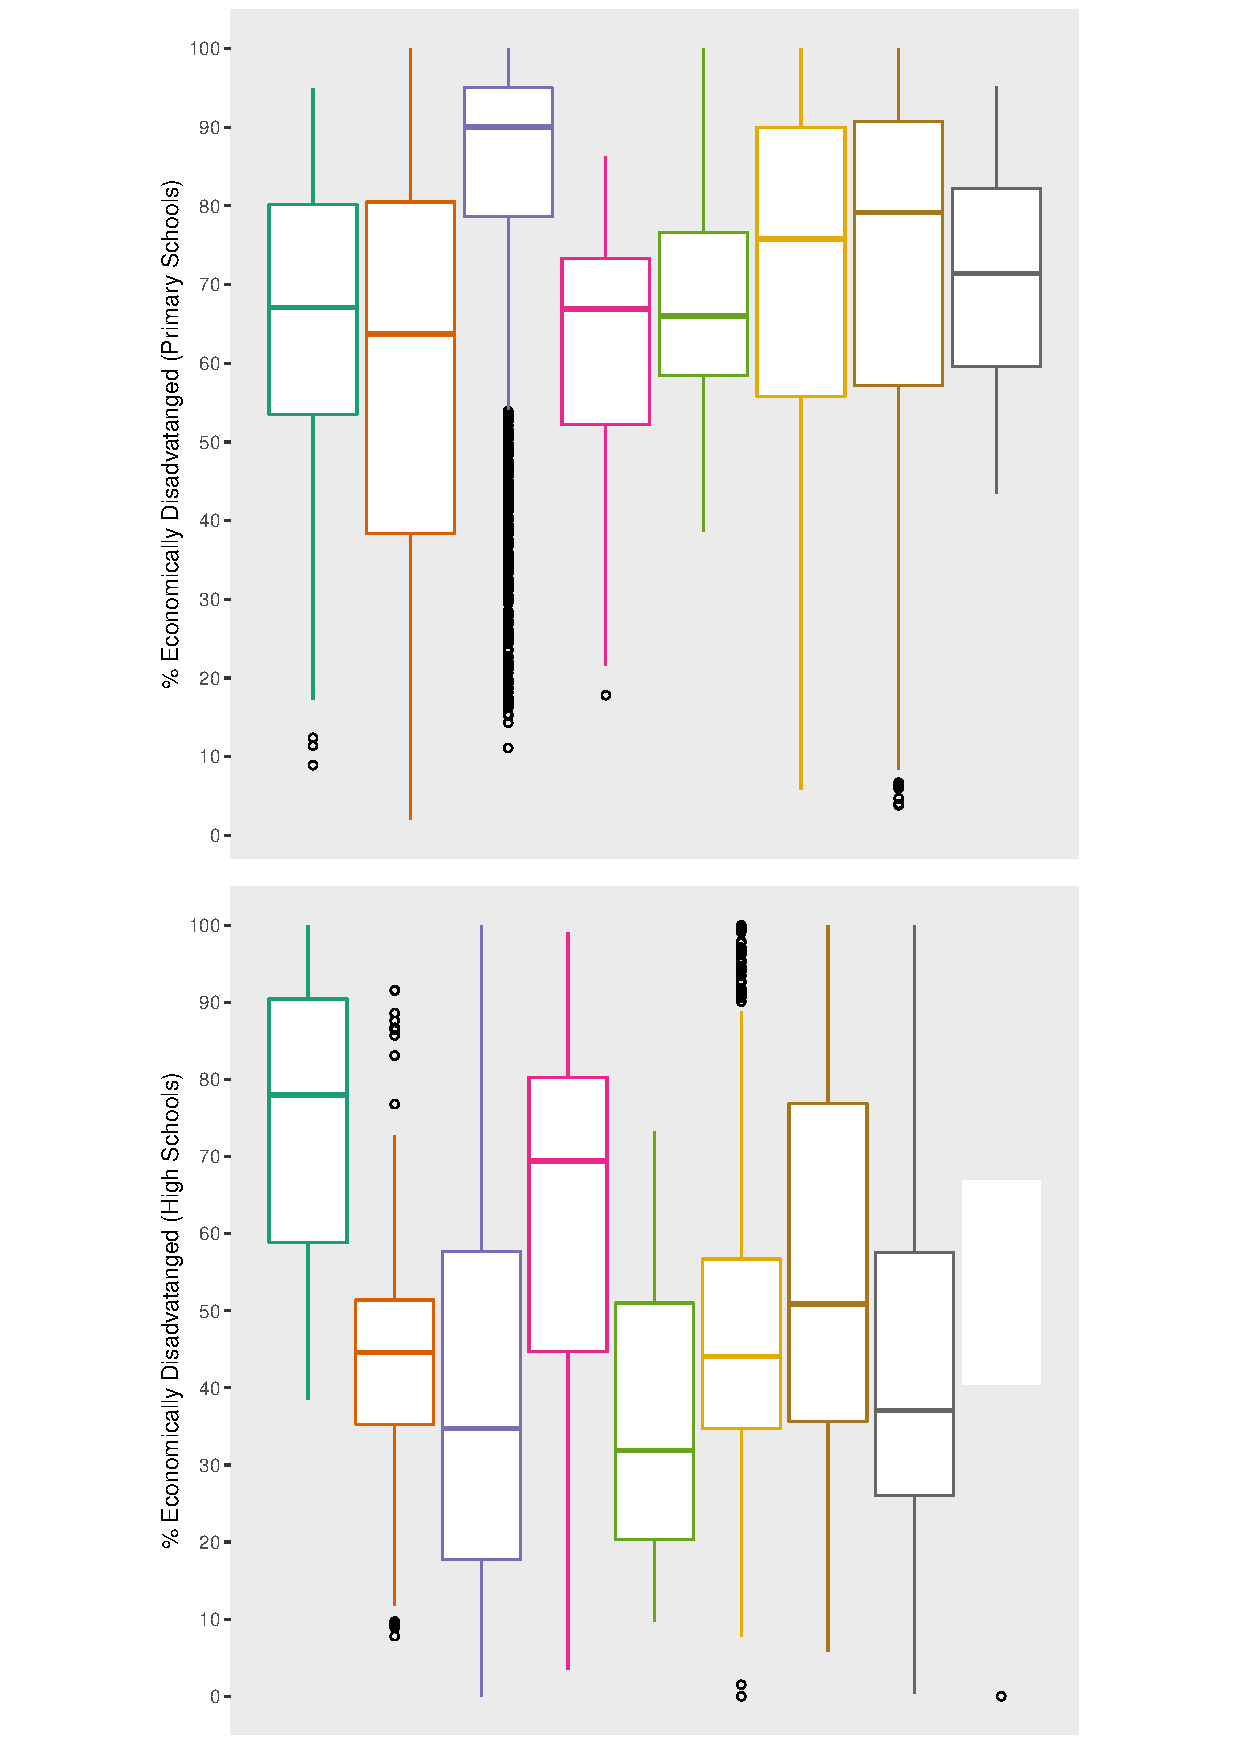
\includegraphics[width=1\textwidth]{/Users/vincentcarse/Desktop/econ_disadv.pdf}
    \includegraphics[width=1\textwidth]{/Users/vincentcarse/Desktop/desc_axis.png}
    \caption{Distribution of economic disadvantage by region. Note the major suburban region is considered relatively 'undeprived' for high schools, but deprived for elementary schools. We will use this, as well as the data on major urban and rural regions to test Lazear's prediction.}
\end{figure}

The results from all four EPFs estimated are not consistent with Hanushek and Rivkin (‘05). Across the 24 different regressions run within the EPF framework, only 1 recorded a negative parameter estimate for per pupil expenditure. This includes the standard OLS regressions run in the first column of the tables. The only evidence in favour of this view came from the IV estimate, where a 1.90 decrease in the 10th grade English pass rate was associated with a \$1000 increase in per student spending, significant at the 0.1\% level. However even in this regression math scores showed no significant effect. 

Lazear's prediction finds some support in the contrast of class size parameters between the 'Major Suburban' and 'Major Urban' regions in the EPFs. As seen in Figure 10, elementary suburban schools are more deprived relative to elementary urban schools, but suburban high schools are less deprived relative to urban high schools. Thus we should expect to see more significant coefficients for class sizes in suburban elementary schools relative to urban elementary schools, but less significant ones for high schools. This is exactly what we observe. The only caution we must exercise in interpreting this result is that urban elementary schools have a very small sample size (81, relative to 2722 suburban ones), so our 5th grade results may be affected by high standard errors.

Most crucially, we find evidence in favour of Hanushek ('97) when adjudicating between the meta-studies. The EPFs find estimates of a decrease between 0.544-1.35 in average pass rates per ten extra students, per pupil expenditure estimates all significant at the 5\% level ranging between 0.39-1.1 pass rate increase per \$1000 per student and failing to reject that teacher salaries and teacher experience are statistically insignificant for maths at grades 5 and 10 and English at grade 10 at the 5\% level. The 'capped' approach estimated a 2.02-2.84 decrease in 5th grade pass rates associated with a \$1000 increase in per student spending, significant at the 0.1\% level. Further to this, the 'Oil IV' approach estimated an insignificant effect on 10th grade math scores, but a 1.90 decrease in the 10th grade English pass rate associated with a \$1000 increase in per student spending, significant at the 0.1\% level. The statistical significance of these estimates varied dramatically, but none were of economic significance. The expenditure parameter would require tens of thousands extra to be spent to gain significance by any estimate. Texans spend an average of \$6,081 per student, so this is clearly infeasible. The class size parameter would require dozens fewer students. 

Tiebout ('56) does not feature directly in this paper, but the limited evidence we do find suggests that proximity to other schools is negatively associated with performance. 

\begin{figure}
    \label{image-myimage}
    \includegraphics[width=1\textwidth]{/Users/vincentcarse/Desktop/eng_reg_gr5.pdf}
    \caption{EPF approach for 5th grade English scores}
\end{figure}

\begin{figure}
    \label{image-myimage}
    \includegraphics[width=1\textwidth]{/Users/vincentcarse/Desktop/math_reg_gr5.pdf}
    \caption{EPF approach for 5th grade math scores}
\end{figure}



\begin{figure}
    \label{image-myimage}
    \includegraphics[width=1\textwidth]{/Users/vincentcarse/Desktop/eng_reg_gr10.pdf}
    \caption{EPF approach for 10th grade English scores}
\end{figure}

\begin{figure}
    \label{image-myimage}
    \includegraphics[width=1\textwidth]{/Users/vincentcarse/Desktop/math_reg_gr10.pdf}
    \caption{EPF approach for 10th grade math scores}
\end{figure}

\begin{figure}
    \label{image-myimage}
    \includegraphics[width=1\textwidth]{/Users/vincentcarse/Desktop/iv.pdf}
    \caption{IV approach for 10th grade scores}
\end{figure}

\begin{figure}
    \label{image-myimage}
    \includegraphics[width=1\textwidth]{/Users/vincentcarse/Desktop/prox.pdf}
    \caption{District proximity effects. An interesting point of departure to test Tiebout's theory.}
\end{figure}

\begin{figure}
    \label{image-myimage}
    \includegraphics[width=1\textwidth]{/Users/vincentcarse/Desktop/capped.pdf}
    \caption{Capped appraoch for 5th grade scores}
\end{figure}


\FloatBarrier

\section{Conclusion}

Education in Texas remains a quagmire of litigation and inefficiency. With tens of billions redistributed for the purpose of education, one hopes funding has a significant impact on performance. This paper found evidence in support of the literature that resource effects on performance are minimal. In particular these were estimates of a decrease between 0.544-1.35 in average pass rates per ten extra students, per pupil expenditure estimates all significant at the 5\% level ranging between 0.39-1.1 pass rate increase per \$1000 per student and failing to reject that teacher salaries and teacher experience are statistically insignificant for maths at grades 5 and 10 and English at grade 10 at the 5\% level. Two alternate identification strategies are also discussed to estimate the causal impact of class size on performance. The 'capped' approach estimated a 2.02-2.84 decrease in 5th grade pass rates associated with a \$1000 increase in per student spending, significant at the 0.1\% level. Further to this, the 'Oil IV' approach estimated an insignificant effect on 10th grade math scores, but a 1.90 decrease in the 10th grade English pass rate associated with a \$1000 increase in per student spending, significant at the 0.1\% level. The statistical significance of these estimates varied dramatically, but none were of economic significance\footnote{The expenditure parameter would require tens of thousands extra to be spent to gain significance by any estimate. Texans spend an average of \$6,081 per student, so this is clearly infeasible}. While these results fit with one vocal side of the education policy debate\footnote{Hanushek ('97)} they leave much to be desired. Further data on historical family, community and school inputs are all still necessary in future studies. With these data, a more realistic educational production can be estimated, taking into account the complex relationships between the inputs into it. Moreover, further avenues of investigation remain open in this topic. Both an oil-value IV approach and a revenue-cap RD approach appear to show promise in identifying causal impacts of resources on test performance, but require further interrogation to be made credible in the eyes of economists. 






\makeatletter
\renewcommand\@biblabel[1]{}
\makeatother

\begin{thebibliography}{9}

\bibitem{2} 
Chetty, Raj; Hendren, Nathaniel;  Kline, Patrick and Saez, Emmanuel, 2014.
"Where is the Land of Opportunity? The Geography of Intergenerational Mobility in the United States",
\textit{The Quarterly Journal of Economics}, (2014) 129 (4): 1553-1623. 

\bibitem{2} 
Coleman, James S., 1966.
"Equality of Educational Opportunity Study",
\textit{Inter-university Consortium for Political and Social Research}

\bibitem{2} 
Cullen, Julie Berry, 2003. 
"The Impact of Fiscal Incentives on Student Disability Rates", 
\textit{Journal of Public Economics}, 87(7-8):1557-89.

\bibitem{2} 
Greenwald, Rob, Hedges, Larry V.  and Laine, Richard D., 1956.
"The Effect of School Resources on Student Achievement",
\textit{Review of Educational Research}, Vol. 66, No. 3 (Autumn, 1996), pp. 361-396 (36 pages)

\bibitem{2} 
Hanushek, Eric A., 1997.
"Assessing the Effects of School Resources on Student Performance: An Update",
\textit{Educational Evaluation and Policy Analysis}, 19(2) Pages: pp. 141-164

\bibitem{2} 
Hanushek, Eric and  Rivkin, Steven G., 2012.
The Distribution of Teacher Quality and Implications for Policy",
\textit{Annual Review of Economics}, 2012, vol. 4, issue 1, 131-157

\bibitem{2} 
 Hoxby, Caroline M., 2001.
"All School Finance Equalizations Are Not Created Equal",
\textit{Quarterly Journal of Economics}, Vol. 116, No. 4 (November), 1189-1231.

\bibitem{2} 
 Hoxby, Caroline M and Kuziemko, Ilyana, 2004.
"Robin Hood and His Not-So-Merry Plan: Capitalization and the Self-Destruction of Texas' School Finance Equalization Plan",
\textit{NBER}, Working Paper No. 10722

\bibitem{2} 
Kane, Thomas J. and Staiger, Douglas O. , 2008.
"Estimating Teacher Impacts on Student Achievement: An Experimental Evaluation",
\textit{NBER}, Working Paper No. 14607

\bibitem{2} 
Krueger, Alan B., 1999.
"Experimental Estimates of Education Production Functions",
\textit{Quarterly Journal of Economics}, Vol. 114, no. 2 (May 1999): 497-532

\bibitem{2} 
Lazear, Edward P. 2001.
"Educational Production",
\textit{The Quarterly Journal of Economics}, Volume 116, Issue 3, August 2001, Pages 777–803,

\bibitem{2} 
Rothstein, Jesse, 2008.
"Teacher Quality In Educational Production: Tracking, Decay, And Student Achievement",
\textit{NBER}, Working Paper 14442


\bibitem{2} 
Steven G. Rivkin, Eric A. Hanushek and John F. Kain, 2005. 
"Teachers, Schools, and Academic Achievement," 
\textit{Econometrica}, Econometric Society, vol. 73(2), pages 417-458, 03.


\bibitem{2} 
Texas Education Agency, Division of Performance Reporting, 2019-20,
\textit{Academic Excellence Indicator System}, 2002-03 to 2010-11. Electronic files.

\bibitem{2} 
Texas Education Agency, Division of Performance Reporting, 2019-20,
\textit{Public Education Information Management System }, 2002-03 to 2010-11. Electronic files.

\bibitem{2} 
Tiebout, Charles M., 1956.
"A Pure Theory of Local Expenditures",
\textit{Journal of Political Economy}, Vol. 64, No. 5 (Oct., 1956), pp. 416-424 (9 pages)

\bibitem{2} 
Todd, Petra E. and Wolpin, Kenneth I., 2003.
"On The Specification and Estimation of The Production Function for Cognitive Achievement",
\textit{The Economic Journal}, 113(485):3-3 · February 2003





 



\end{thebibliography}




\end{document}

